\section{Method}

\begin{figure}
    \centering
    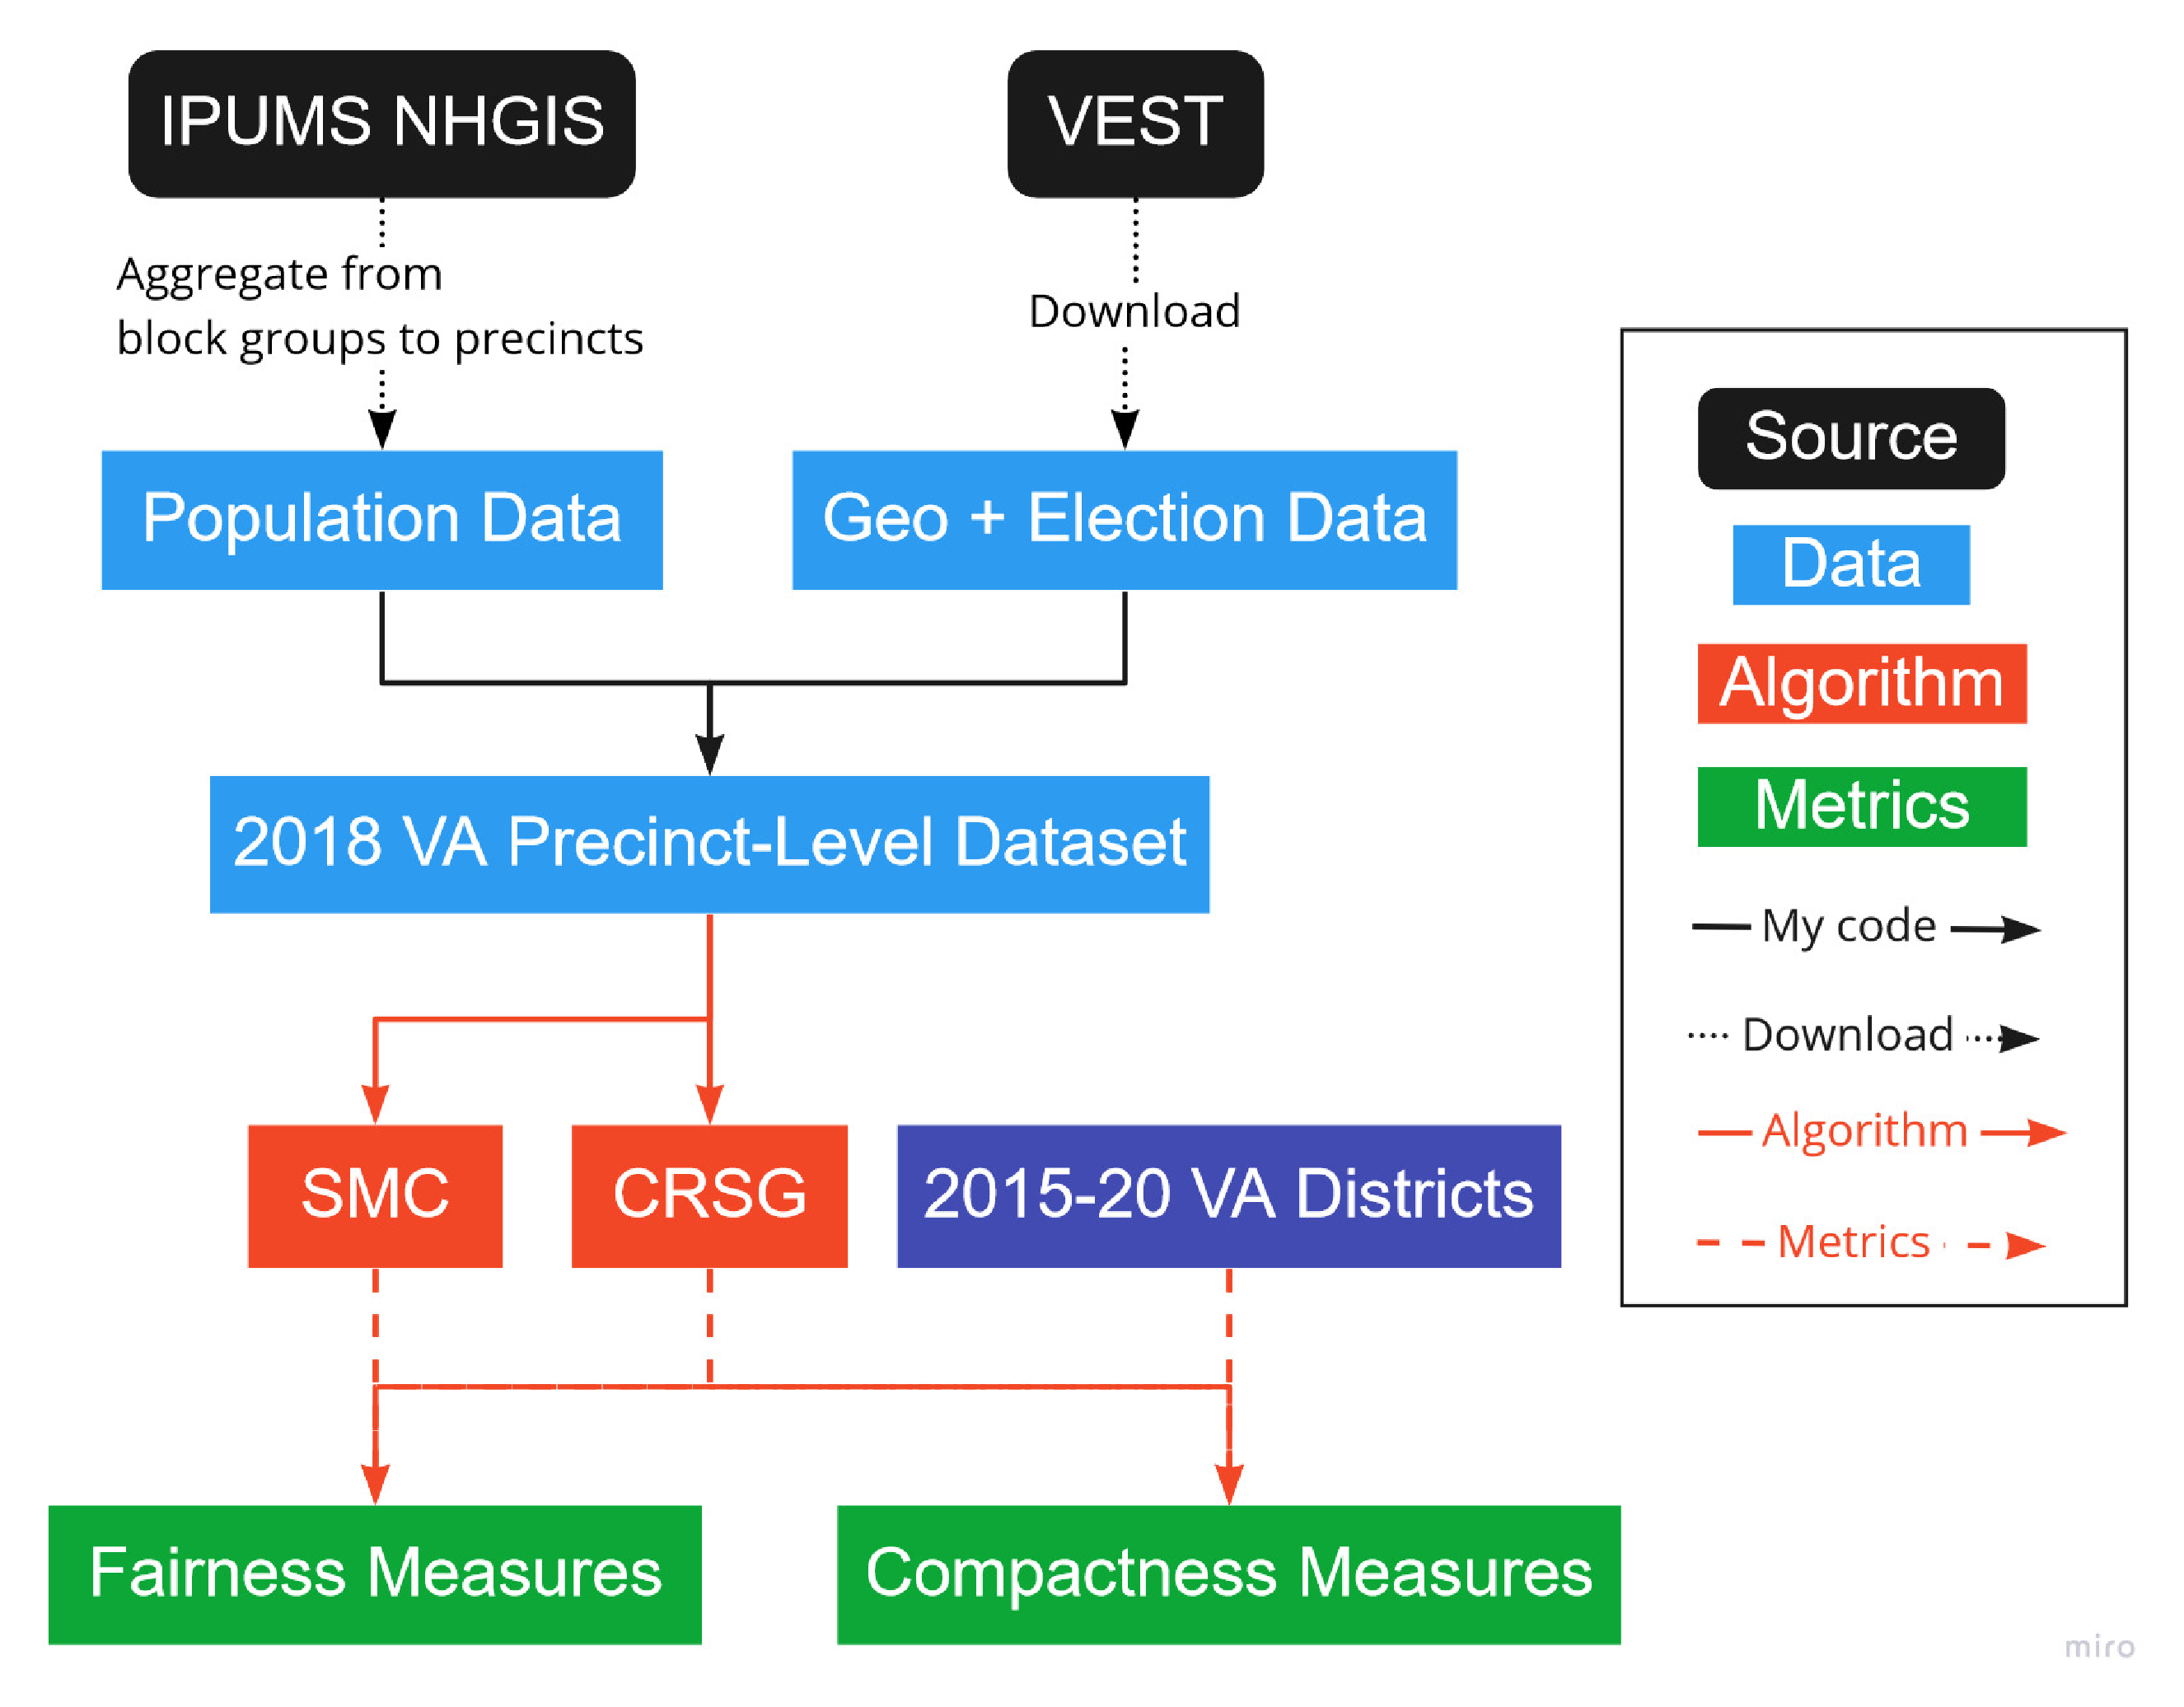
\includegraphics[width=0.6\linewidth]{img/flowchart.pdf}
    \caption{Graphical Overview of project}
    \label{fig:flowchart}
\end{figure}

My research method simulates the 2020 redistricting of the congressional districts in Virginia using two different algorithms supplied with data from 2018. Figure \ref{fig:flowchart} provides and overview of this process.

\subsection{Choice of Research Method}

For this study, I chose to use the experimental design method because it will allow me to isolate the hypothetical impact of the redistricting algorithm from other possible confounding variables. This method also includes the use of a control group, which allows the researcher to establish causation. 

\subsubsection{Components of Experimental Design}

\paragraph{Experimental Units}

The experimental units for this study are the complete datasets for each election year in Virginia.\footnote{This corresponds to the blue rectangles in Figure \ref{fig:flowchart}.} Every row in each dataset corresponds to a precinct, the smallest geographical unit by which votes are tabulated in Virginia. For each precinct, I also have the total population and the number of votes cast for the 2018 Democrat, Republican, and other congressional candidates.  Additionally, each precinct has a polygon associated with it that represents its geographical shape. 

\paragraph{Treatments}

The treatments for this study are the two different redistricting algorithm that I'm comparing: Markov chain Monte Carlo \parencite{fifield2020} and Sequential Monte Carlo \parencite{mccartan2020}.\footnote{This corresponds to the red rectangles in Figure \ref{fig:flowchart}} I'm using the implementations in the R programming language "redist" package \parencite{fifield2020d}. See the Literature Review for more information . Broadly, I chose them because they are deterministic. Much of the literature focuses on creating many possible redistricting plans for a commission to choose from, but these three aim to create an "ideal" map. A redistricting plan generated by CRSG serves as the initial map for the MCMC algorithm.\footnote{MCMC requires a valid map to start with, and the existing map of Virginia was not valid as the population parity was no longer within 1\%, as the population has changed since 2016 when the map was drawn.} 

\paragraph{Response Variables}

Broadly, the goal will be to evaluate how "fair" and compact each redistricting plan generated by each algorithm for each year is.\footnote{This corresponds to the green rectangles in Figure \ref{fig:flowchart}.} Refer to the Literature Review for more information on the fairness and compactness measures chosen.

\subparagraph{Compactness Measures}

I chose to compute the mean Polsby-Popper score, Fryer-Holden score, and the Edge-Cut Compactness measure for the proposed maps from each algorithm. I did not have the necessary computational resources to compute all of the measures that I describe in my Literature Review, so I elected to compute the most popular area-based measure (Polsby-Popper), the only population-based measure (Fryer-Holden), and the primary graph-theory measure (Edge Cut Compactness). While not complete, these measures provide a representative overview of the possible compactness measures. 

\subparagraph{Fairness Measures}

I chose to compute the Partisan Bias, Declination, Efficiency Gap, Equal Population Efficiency Gap, Lopsided Wins, Mean-Median, Responsiveness, and Tau Gap measures, all of which are described in the Literature Review, as they represent the fairness measures discussed at present in the literature \parencite{katz2020}. Computational resources were not a barrier for this step, so I was able to calculate all of the measures. 

\subparagraph{Chamber Power Balance}

Since the redistricting that's occurring is hypothetical and I have precinct-level election results for each of these years, I also simulate how many seats the Democratic party would have won in the 2018 General Election under the various redistricting plans. 

\paragraph{Control Group}

The official VA Congressional district map used in the years 2016-2020\footnote{Due to racial gerrymandering, VA had to adopt a new congressional district map in the middle of the decade \parencite{breyer2016}.} will serve as the control group for this experiment. I will compute the same metrics for this map as I will for my hypothetical redistricting plans.\footnote{This corresponds to the purple rectangle in Figure \ref{fig:flowchart}.}

\subsubsection{Principles of Experimental Design}

The primary principles of experimental research design are randomization, replication, and local control. This is how I plan to address them. 

\paragraph{Randomization}

Every experimental unit will receive each treatment, and every experimental unit can be replicated many times without issue, so there’s no error from a lack of randomization. Think of each treatment operating within a separate parallel universe. 

\paragraph{Replication}

Each algorithm will generate 100 sample redistricting plans. This is large enough to allow for inferences, but small enough to still be computationally feasible. 

\paragraph{Local Control}

All of the redistricting will be happening in controlled environments, so there will be no way for lurking variables to creep in and confound my results. 

\subsection{Data Cleaning}

To create my datasets, I cleaned and compiled three different types of data: demographic data, Geographic Information Systems (GIS) data, and election data.\footnote{This is an explanation of the black and blue rectangles in Figure \ref{fig:flowchart} and the transitions between them.} 

\subsubsection{Demographic Data}

One required piece of data in order to redistrict is demographic data at the precinct level. For my purposes, this means the total population of each precinct. In order to run the most accurate redistricting simulations, these data needed to be recent for the year being redistricted. Comprehensive population counts are only conducted by the US Census Bureau every 10 years, so I instead used the 5-year American Community Survey results at the block-group level. This is a sample survey, not a population count, but that is offset by the aggregation of sample data over a 5 year period. I downloaded this data from the IPUMS National Historic GIS project \parencite{mansonsteven2020}. Using the "maup" Python Library \parencite{hully}, I disaggregated the data from the block-group level to the block level, prorating the demographic data based on population. This data was then aggregated up to the precinct level.

\subsubsection{GIS Data}

In order to redistrict, the algorithms need to know the shape and relative location of each precinct. In practice, this means every precinct has a "polygon" associated with it and a Coordinate Reference System that describes where these polygons fall in space. These data tables with the geometry column are known as "shapefiles." I accessed these shapefiles from the Voting and Election Science Team on their Harvard Dataverse \parencite{votingandelectionscienceteam2019c}. I then merged in my precinct-level demographic data tables, so I now have shapefiles with the necessary demographic data. \footnote{Since election administrators are free to change the precincts between elections, precinct shapefiles are unique to both a place and a time. This is why I couldn't use the 2018 precinct shapefiles with 2020 election results.}

\subsubsection{Election Data}

The last necessary component needed to evaluate redistricting plans is the number of votes won by each party in each precinct in each election.\footnote{The algorithms I'm comparing assume a 2 party system, so I only tracked Democratic and Republican votes won in each election.} Conveniently, this data was already included in my shapefiles by the Voting and Election Science Team. 